\chapter{Motivación y Antecedentes}
\section{Crecimiento de la red}
El gran crecimiento en la cantidad de sistemas teconológicos interconectados via Internet en el mundo en los últimos 30 años es algo que no ha dejado indiferente a nadie. Para entender este fenómeno, distintos organismos internacionales se dedican periodicamente a realizar estimaciones de dicha cifra. Un caso muy popular de dicha labor es el contador global de conexiones móviles a Internet del GSMA Intelligence\footnote{\url{https://gsmaintelligence.com/}} el cual recientemente ha estimado en más de 7 mil millones el número de dispositivos móviles con conexión a la red, superando por primera vez al total de la población mundial\footnote{\url{http://www.cnet.com/news/there-are-now-more-gadgets-on-earth-than-people/}}. Una premisa que coincide con el último informe \emph{The State Of Internet} de \emph{Akamai} \cite{report:akamai} donde se resume el estudio de las principales variaciones en capacidad de acceso, velocidades de acceso, tipos de ataques, etc. a Internet de que disponen distintos países del mundo. Éste estudio corroboró lo que ya ha sido tendencia en los últimos años: Tanto las velocidades de navegación, así como el total de conexiones a Internet han aumentado generalizadamente en todo el planeta. Las proyecciones a futuro preservan ésta tendencia apostando a que tanto la cantidad de dispositivos como el número de accesos a Internet deberían seguir subiendo \cite{nota:2020}, ello producto de factores como la reducción de costos de producción y la minimización de la tecnología, además de distintas tendencias generadas a raíz del fenómeno de \emph{globalización} que -en gran medida- nos ha forzado a participar de una sociedad más interconectada en todo el mundo y explicarían dicha tendencia. Olvidando un poco las interpretaciones o justificaciones para ésta situación, el hecho concreto es que existe una directa proporcionalidad entre el número de dispositivos y los requerimientos de accesos a la red, y hoy ambos están en su apogeo de crecimiento.

\begin{figure}[!h]
	\centering
	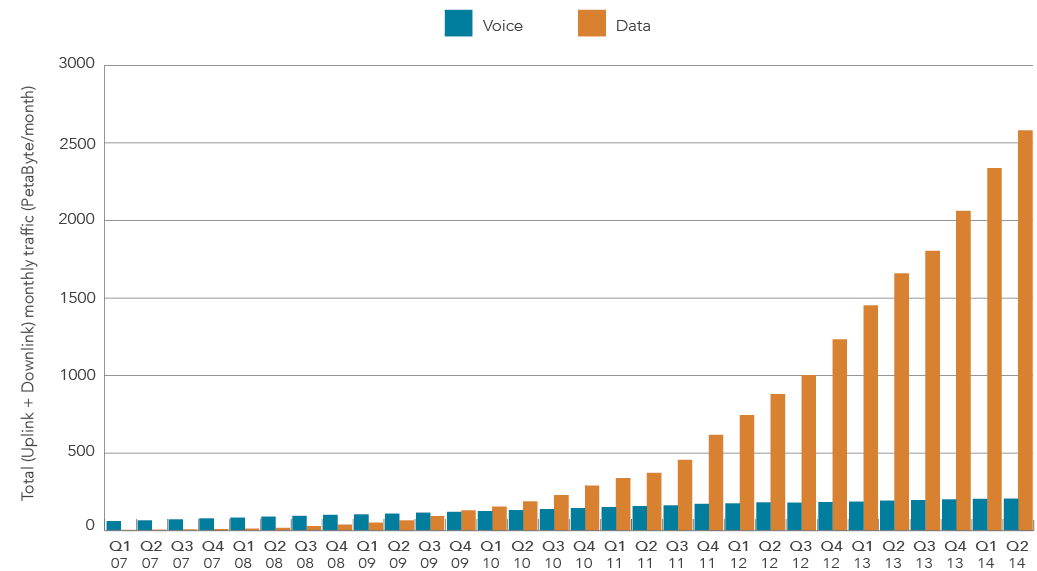
\includegraphics[scale=0.5]{imagenes/conexiones_moviles}
	\caption{Registros de la compañía \emph{Ericsson} ilustrando el crecimiento exponencial en el uso de datos de los dispositivos móviles. Parte del informe de \emph{Akamai} \cite{report:akamai}}
	\label{fig:akamai_stats}
\end{figure}

Más allá del número de dispositivos o la cantidad --o calidad-- del acceso a Internet, las distintas aplicaciones que ha desarrollado la industria han evolucionado sobre la base de protocolos y sistemas diseñados hace varias décadas, exigiendo siempre la mejor performance posible en pos de garantizar buenos tiempos de respuesta. Los protocolos más celebres de la llamada \emph{familia de protocolos de Internet} son TCP e IP. Sin embargo, son decenas los protocolos y mecanísmos involucrados en las diferentes fases de comunicación entre computadoras y aplicaciones, que permiten en conjunto la operación de la red de redes como hoy la conocemos.

\section{El modelo OSI de conexion en Internet}
La capacidad de conectividad entre 2 distintos dispositivos es resultado del efecto combinado de varias capas de abstracción con responsabilidades divididas. Un diseño de operación que se ilustra en un modelo estándar vigente desde los años 80 es el impulsado por la \emph{Organización Internacional de Normalización} (\textbf{ISO}), mejor conocido como el modelo \textbf{OSI} por sus siglas en inglés \emph{Open System Interconnection}. En la práctica, la importancia de éste modelo radica en servir como una referencia técnica que ilustra los límites en las responsabilidades entre componentes que conforman una arquitectura de interconexión de sistemas.

El modelo OSI reconoce 7 capas de abstracción en el proceso de comunicación entre dispositivos, cada una con obligaciones especificas y que juntas, soportan constructivamente un mecanismo de comunicación estándar para sistemas que por él se rijan. El acierto de éste enfoque está en permitir el desarrollo de soluciones modulares y especificas a cada una de las capas, sin interferir entre capas diferentes y manteniendo así la compatibilidad con aplicaciones que ya operen en capas distintas. Las 7 capas en cuestión se describen a continuación:

\begin{figure}[!h]
	\centering
	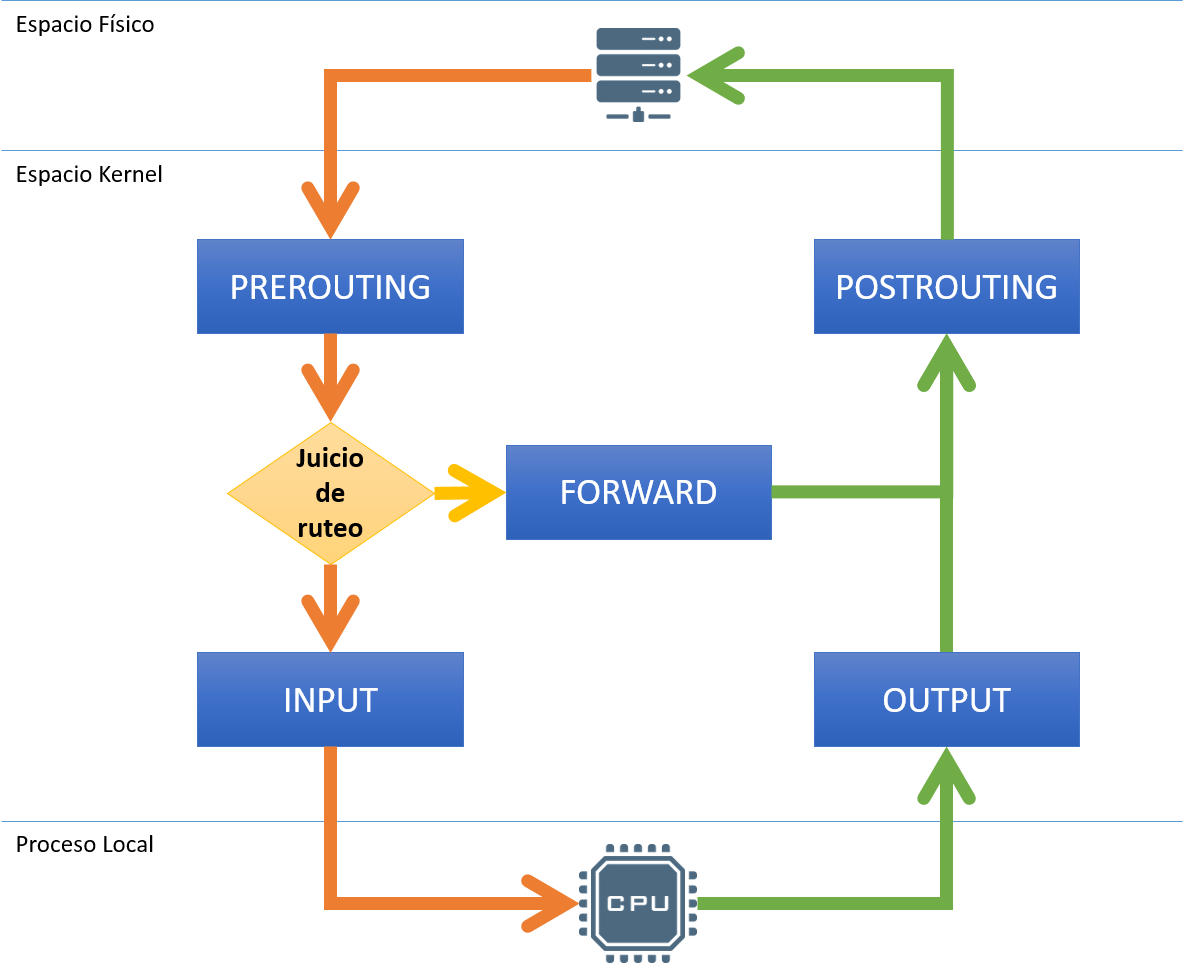
\includegraphics[scale=.3]{imagenes/netfilterArchitecture}
	\caption{Diagrama esquemático de las 7 capas del modelo OSI.}
	\label{netfilterArchitecture}
\end{figure}

\begin{description}
\item[Capa Física] La capa de nivel inferior en el modelo OSI es la capa física. Es ésta capa la responsible de la topología de la red y de la especificación de los medios materiales que consiguen la transmisión de la información, así como también es responsable de la generación real de la comunicación por medio del envío de la información. Es, en definitiva, la encargada del paso a canales físicos de la información a transmitir.

\item[Capa de Enlace] Es la segunda capa del modelo. Ella se encarga de proveer un mecanismo de direccionamiento físico en una máquina que permita el reconocimiento individual de la misma, proveiendo de un primer identificador a las máquinas en el modelo OSI, dado por las direcciones físicas de los dispositivos (\emph{Dirección MAC}). Es responsible también de proveer mecanismos de corrección de errores en el proceso de transmisión de datos que pudiesen manifestarse por problemas de la capa física, haciendo dicha comunicación desde éste punto, confiable.

\item[Capa de Red] Es la tercera capa del modelo. Hace su debut en contextos de multiples equipos interconectados brindando mecanismos de identificación para proveer una capacidad de direccionamiento más amplia con respecto al disponible en las dos primeras capas (que básicamente permitian la comunicación entre un par de máquinas, punto a punto). En éste nivel aparece uno de los protocolos más populares en Internet, el denóminado protocolo IP que supone un mecanismo de identificación único para cada dispositivo en una red, provisto en base a una dirección homónima. Ésta capa establece la capacidad de ruteo en la comunicación como una responsabilidad de los nodos en una infraestructura en red, haciendo cada componente de la red alcanzable para cualquier otro integrante de la misma.

\item[Capa de Transporte] La cuarta capa del modelo, es la que provee de lleno la capacidad de transporte de datos. En éste nivel se incorporan los también celebres protocolos homónimos: TCP (orientado a la conexión) y UDP (orientado a la mensajería). Ésta capa es también responsible de brindar la capacidad de multiplexación a nivel de una máquina, permitiendo la generación de multiples conexiones desde el mismo dispositivo, dicho mecanismo lo consigue al incorporar puertos lógicos de comunicación. De ésta manera, a partir de la capa de Transporte se establece un paradigma base en lo que a programación y esquematización en el area de redes corresponde: La correspondencia sockets \emph{IP:PUERTO}, que conforman finalmente el concepto de tuplas de direccionamiento en el proceso de transporte de datos.

\item[Capa de Sesión] Es la quinta capa del modelo OSI. Tal y como su nombre lo indica su función radica en ser la responsible de mantener un control de sesión en una conexión entre hosts, proveiendo mecanismos de corrección y reconexion en caso de interferencia de una operación entre máquinas. Se encarga de mantener el enlace de comunicación construido en base a las capas inferiores en un proceso de comunicación.

\item[Capa de Presentación] El sexto nivel en el modelo OSI es la capa de presentación, cuya responsabilidad comprende proveer el soporte para dar una correcta interpretación de los datos transmitidos, de manera de conseguir que los datos lleguen de manera reconocible al host de destino. A diferencia de las capas inferiores que se enfocan en los mecanismos de envío de la infromación, ésta capa guarda directa relación con la infromación transmitida y su correcta interpretación.

\item[Capa de Aplicación] Es la última -y de más alto nivel- capa de abstracción del modelo OSI. Es la responsible de proveer una interfaz simple a aplicaciones al acceso a mecanismos de comunicación en red. En otras palabras, es la responsible de proveer el servicio de comunicaciones a las distintas aplicaciones que tengan requerimientos de comunicación.

\end{description}

A pesar de que el modelo OSI plantea responsabilidades delimitadas a cada capa de abstracción, la correspondencia de dicho estándar en la práctica es una labor que queda supeditada a los programadores de sistemas operativos. Finalmente son ellos los que, en mayor o menor medida, hacen corresponder para con el modelo, las implementaciones finales de los módulos de red de un sistema.


\section{Familia de Protocolos de Internet}
El conjunto de múltiples protocolos que facultan a los sistemas de mecanismos de interconexión comprende a varios cientos que se distribuyen entre las distintas capas del modelo OSI. A Este conjunto se le denomina \emph{Familia de Protocolos de Internet}. Sin embargo, historicamente se le ha prestado especial atención a un subconjunto de ellos que son estructurales en la infraestructura en Internet y que rigen la misma, hablamos del conjunto de protocolos \textbf{TCP/IP}.

La arquitectura del protocolo TCP/IP sigue la inspiración del modelo OSI en las responsabilidades a soportar, a pesar de romper la estructura de capas del mismo, combinando algunas responsabilidades de dicho modelo en funciones únicas y obviando otras. PAra un ejemplo de esto, se puede ver la tabla \ref{tabla:tcpiposi} que ilustra la correspondencia de los protocolos TCP/IP con su atribución según el modelo OSI.

\begin{table}[h!]
\centering
\begin{tabular}{|c|p{4cm}|l|p{5cm}|}
\hline
\multicolumn{1}{|c|}{\textbf{\begin{tabular}[c]{@{}c@{}}Ref. OSI\\ Nº de capa\end{tabular}}} & \multicolumn{1}{c|}{\textbf{\begin{tabular}[c]{@{}c@{}}Equivalente \\ de capa OSI\end{tabular}}} & \multicolumn{1}{c|}{\textbf{Capa TCP/IP}} & \multicolumn{1}{c|}{\textbf{\begin{tabular}[c]{@{}c@{}}Ejemplos de\\ protocolos TCP/IP\end{tabular}}} \\ \hline
5,6,7                                                                                        & Aplicación, Sesión, Presentación                                                                 & Aplicación                                & NFS, NIS, DNS, LDAP, telnet, ftp, rlogin, rsh, rcp, RIP, RDISC, SNMP y otros.                         \\ \hline
4                                                                                            & Transporte                                                                                       & Transporte                                & TCP, UDP, SCTP                                                                                        \\ \hline
3                                                                                            & Red                                                                                              & Internet                                  & IPv4, IPv6, ARP, ICMP                                                                                 \\ \hline
2                                                                                            & Vínculo de datos                                                                                 & Vínculo de datos                          & PPP, IEEE 802.2                                                                                       \\ \hline
1                                                                                            & Física                                                                                           & Red física                                & Ethernet (IEEE 802.3), Token Ring, RS-232, FDDI y otros.                                              \\ \hline
\end{tabular}
\caption{acá la tabla de comparaciones. La robé desde \url{https://docs.oracle.com/cd/E19957-01/820-2981/6nei0r0r9/index.html}}
\label{tabla:tcpiposi}
\end{table}


\subsection{UDP}
UDP \cite{rfc:udp} es un protocolo de la familia de protocolos de Internet con funciones a nivel de la capa de transporte según el modelo OSI que se caracteriza por ser un protocolo orientado a mensajes, vale decir, por permitir enviar mensajes a través de la red sin necesidad de establecer previamente una conexión con el equipo receptor (situación que si ocurre y es característica de los protocolos orientados a la conexión como es el caso de TCP).
%[OSI reference model—The ISO model of architecture for open systems interconnection]%

Ésta naturaleza de UDP tiene varias implicancias:
\begin{itemize}
\item En primer lugar, ser un protocolo orientado a mensajes supone una premura en el envío de información, ello significa que éste protocolo no verifica la correctitud en la recepción de los datos enviados. En ese sentido, UDP es lo que se denomina un protocolo \textbf{no fiable}.
\item Por otro lado, UDP trabaja en estados denominados \textbf{sin conexión}, lo que significa que no hay una verdadera sincronización entre origen y destino. Esto supone el uso de operaciones del tipo asíncronas las que hacen más flexible la comunicación entre los extremos.
\end{itemize}

Por su funcionamiento, la anatomía o estructura de un paquete UDP es bastante simple (Ver fig. \ref{fig:datagramaudp}). Al ser un protocolo orientado al envío de mensajes, los paquetes disponen de pocos campos de e información, de manera de evitar sobrecargar los mismos en su transferencia, por ello, a éste nivel, los paquetes se denominan \emph{datagramas}. Los encabezados de un paquete UDP comprenden: \textbf{Puerto de Origen/Destino}, que hace referencia a los puntos de conexión de la capa Transporte del modelo OSI y \textbf{Longitud del Mensaje} y \textbf{\emph{Checksum}}\footnote{Corresponde a un valor generado a partir de una función matemática que se aplica sobre datos para corroborar la integridad de los mismos y su correcta recepción tras un envío.}, que sirven como componentes de verificación del paquete mismo.

\begin{figure}[!h]
	\centering
	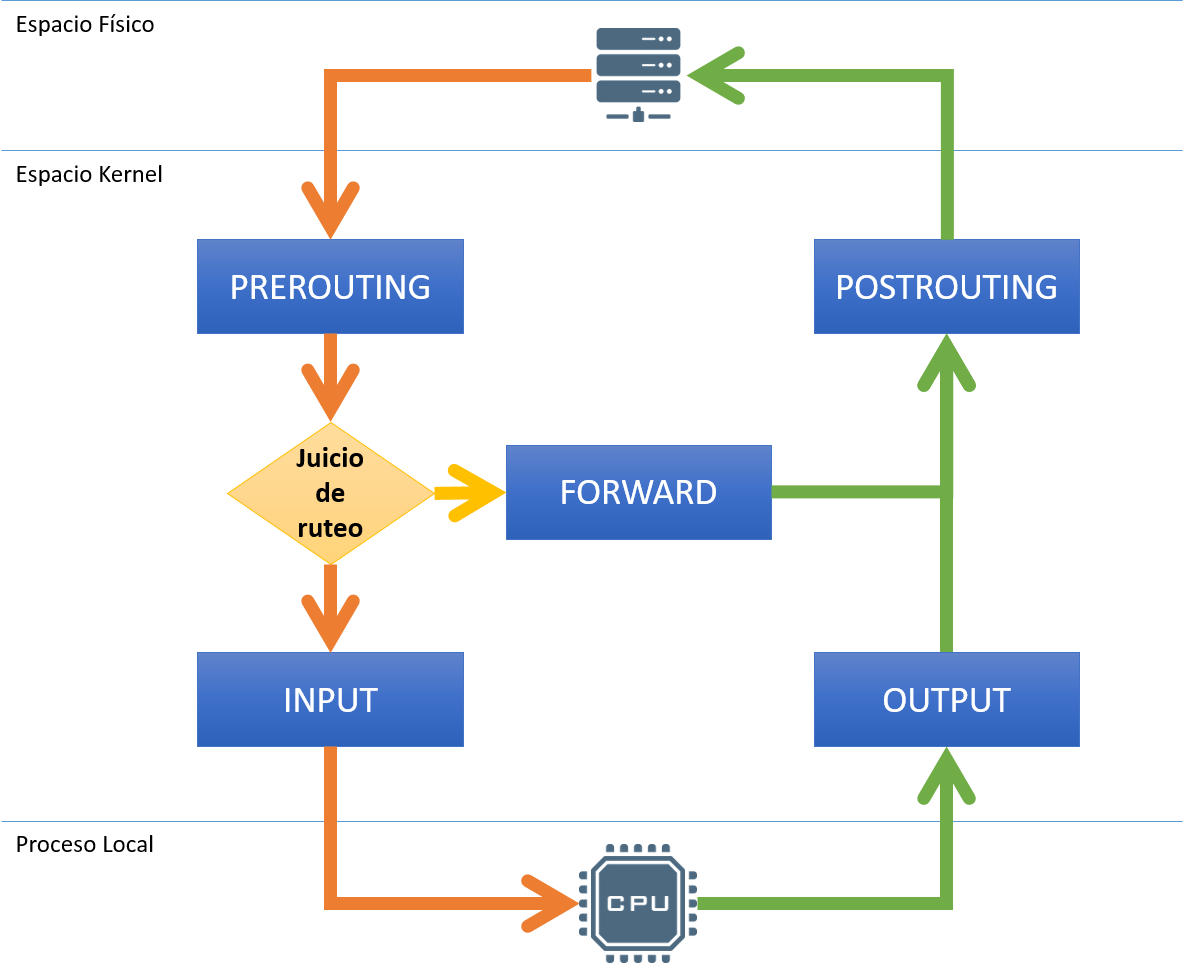
\includegraphics[scale=.3]{imagenes/netfilterArchitecture}
	\caption{Estructura de un paquete UDP.}
	\label{fig:datagramaudp}
\end{figure}

El protocolo UDP se estandarizó el año 1980 \cite{rfc:udp}, siendo uno de los componentes estructurales en la Internet de hoy, estando presente en diversas aplicaciones como: Transmisiones en uso intensivo de datos para redes de alta velocidad \cite{udp:highbandwidth}, Mecanismos de transmisión de video \cite{udp:video}, entre otros. Sin embargo, una de las aplicaciones más importantes que utiliza éste protocolo hoy por hoy en la infraestructura de Internet es en el servicio DNS.

\subsection{DNS}
Todo dispositivo conectado a una red de computadoras se identifica a si mismo por la denominada \emph{dirección IP}, un identificador único que permite referenciarlo y diferenciarlo de otros dispositivos conectados a la misma red, definido por el nivel 4 de red del modelo OSI. No obstante, para poder conectarse con un recurso disponible en Internet, los dispositivos consultan por lo que llamamos \emph{nombres de dominio} que son identificadores con carácter semántico para los usuarios que, en estricto rigor, definen una red de identificación asociada a un grupo de dispositivos o equipos conectados a la red \cite{wiki:nombre_dominio}. Éste mecanismo de traducciones se conoce como \textbf{servicio DNS} y es vital para el funcionamiento de Internet como lo conocemos.

El servicio DNS opera como una base de datos distribuida que permite resolver consultas de manera jerarquizada. Frente a una consulta de un cliente por un nombre de dominio, un servidor DNS puede tener la respuesta, en cuyo caso éste servidor responde sin mayores inconvenientes. En caso contrario, dicho servidor DNS promueve la consulta a un servidor DNS de mayor rango en la jerarquía DNS hasta alguno que conozca la IP asociada al nombre de dominio consultado. Eventualmente, si ninguno de los servidores intermediarios conoce la respuesta, la consulta llega a los servidores raíz, de los cuales se responde la consulta ya sea con la respuesta efectiva o con la información de que el registro no existe (ver figura \ref{fig:dns}).

\begin{figure}[!h]
	\centering
	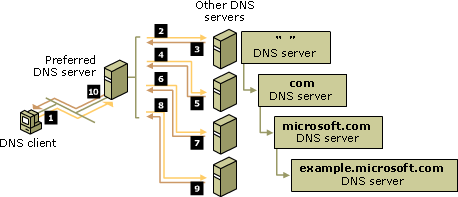
\includegraphics[scale=0.7]{imagenes/dns-system}
	\caption{Diagrama de operación del servicio DNS ilustrando comunicación entre servidores de dicho tipo.}
	\label{fig:dns}
\end{figure}

En la práctica, el servicio DNS emplea el protocolo UDP para la comunicación desde y hacia los servidores de dicho tipo, esto pues las características de una consulta DNS contemplan:

\begin{itemize}
\item \textbf{Consultas Auto-Contenidas} La información de una consulta DNS calza fácilmente en un paquete de UDP.
\item \textbf{Orden Irrelevante} Los requerimientos DNS no necesitan ser procesados en un orden establecido. Sin embargo, si requieren ser eventualmente procesados y ello en el menor tiempo posible. Un factor que justifica el uso de UDP al ser precisamente un protocolo orientado a mensajes.
\end{itemize}

De esta manera, las características anteriores justifican el uso de UDP como protocolo para la comunicación entre los servidores DNS.

El escenario antes descrito explica porque UDP tiene una participación de gran importancia en las redes actuales (en especial sobre Internet) y además, dado el sostenido aumento en el número de conexiones explicado en las secciones previas, da cuenta de como el tráfico de éste tipo de comunicación representa una porción muy significativa en la operación de las redes modernas.

\section{Sistemas Operativos Modernos}
capacidad multiprocesador!

\subsection{Mecanismos de Sincronización}
Una responsabilidad fundamental de los sistemas operativos modernos es asignar el uso de recursos a las aplicaciones y garantiar un entorno seguro para la ejecución de dichas aplicaciones, en el sentido del acceso a datos o recursos del sistema. En ésta linea, garantizar \textbf{consistencia en los datos} es una labor crucial en esquemas modernos, capaces de generar escenarios de multiples aplicaciones con acceso simultáneo a datos compartidos entre ellas. La característica de operaciones paralelas es una introducción al kernel de Linux desde su versión 2.6\footnote{En versiones previas del kernel, la operación por defecto del scheduller del kernel era serializar las tareas con accesos simultaneos al sistema.} [AKA REF], lo cual introdujo un nuevo nivel de complejidad al ser responsables de éste nuevo escenario.

Para proveer operaciones sobre los datos en escenarios concurrentes, los sistemas operativos implementan mecanismos de sincronización que permiten garantizar consistencia en sus estructuras y datos, permitiendo así operaciones "simultaneas" sobre una determinada estructura, permitiendo incluso compartir una estructura entre distintos procesos que la modifiquen coincidentemente.

Hablar de los distintos tipos de mecanismos de sincronizacion de datos.

\subsection{Interfaces de Comunicación}

Aka no he puesto nada aún...

\subsection{Sockets en Linux}
El modelo OSI ha estipulado a la familia de los protocolos TCP/IP como un estándar a la hora de establecer mecanismos de conexión entre computadoras. Sin embargo, las interfaces de programación no siguen la misma naturaleza estándar. Los distintos sistemas operativos implementan distintas interfaces públicas de aplicación (API) para el uso práctico de TCP/IP. \textbf{Socket} es la denominación tradicional para las interfaces de programación que proveen los mecanísmos para realizar tales conexiones. En la práctica un \textbf{Socket} representa una interfaz o punto de comunicación que maneja un protocolo de comunicación especifico. En la práctica, los sockets operan bajo una dinámica denominada \emph{Cliente/Servidor}, que especifíca que la comunicación debe ser promovida inicialmente por un cliente y atendida por un servidor.

Los sockets son estructuras que se construyen por medio de la llamada de sistema \verb=socket()=. Son estructuras provistas por el kernel del sistema\footnote{Típicamente implementada e importada desde el prototipo \verb=<sys/socket.h>=, disponible en los encabezados del kernel.} que al utilizarlos se manejan simplemente como descriptores de archivo, a pesar de que en su implementación a bajo nivel son bastante más complejos que una interfaz de sólo entrada y salida de datos. La gran diferencia de los sockets es que están concebidos para una operación basada en un principio \emph{Cliente-Servidor}, lo que impacta finalmente en que su descriptor no apunta directamente a un archivo y su utilidad queda determinada sólo desde el momento en que se complete la dinámica de llamadas a sistema que hagan se establezca una conexión efectiva, dependiendo del protocolo a usar (ver imagen \ref{fig:socketHandshake}). Linux cuenta con una API que provee métodos de comunicación sencillos para la maniulación de los sockets de acuerdo al protocolo para el que se configure el mismo.

\begin{figure}[h!]
	\centering
	\subfigure[Llamadas de sistema en conexión TCP]{
		
\includegraphics[width=.4\textwidth]{imagenes/fcfm}
	}
	\subfigure[Llamadas de sistema en conexión UDP]{
		
\includegraphics[width=.4\textwidth]{imagenes/fcfm}
	}
	\caption{Un esquemático de las llamadas a sistema que se deben suceder para establecer una conexión.}
	\label{fig:socketHandshake}
\end{figure}

El sistema operativo reconoce a los diferentes sockets en operación a través de sus detalles de conexión de red, ello por medio de tuplas que contienen información de la conexión que provee el mismo. Una tupla congrega datos como: El protocolo de comunicación, las direcciones local y remota (con datos de las capas de red y de transporte para la identificación del punto de acceso: IP:PUERTO) y los identificadores de procesos local y remoto propietarios del punto de comunicación.

\begin{verbatim}
{Protocolo, dirección_local, proceso_local, dirección_remota, proceso_remoto}
\end{verbatim}

Los sockets son elementos muy versátiles en cuanto a su manipulación y uso. Se pueden usar en dos variantes principales que determinan el \emph{dominio del socket}:
\begin{description}
\item[Unix Sockets] Una descripcion de los unix socket
\item[Internet Sockets] Una descripcion de los internet socket socket.
\end{description}

Para las variedades recien mencionadas hay que sumar la capacidad de configuración de un socket. La primera y más importante es la configuración del modo de conexión que regirá la dinámica de comunicación del socket: El \emph{protocolo de comunicación}. En éste apartado existen dos variantes comúnmente usadas: \textbf{SOCK\_STREAM} y \textbf{SOCK\_DGRAM} para usar TCP o UDP respectivamente. Sumado a lo anterior, los sistemas Linux proveen de la llamada de sistema \verb=setsockopt= que permite modificar características de una instancia socket, activando ciertas funcionalidades especificas o habilitando variedades de la implementación original con modificaciones especiales con respecto al funcionamiento estándar.

Más allá de la configuración puntual de la que se dote a un socket, la estructura interna de éste elemento es estándar y tiene especificaciones importantes de comentar para comprender su funcionamiento y posibles limitaciones.

\subsubsection{Estructura Interna}

\section{Presentación del Problema}
Como ya se mencionó, el escenario advertido para los próximos años prevé un inmenso tráfico a Internet que podría llevar la cantidad de procesamiento del servicio DNS a varios órdenes de magnitud por encima de la carga actual. Es más, el panorama futuro propone que los dispositivos más avanzados serían muchísimo más versátiles en su operación pudiendo hacer un uso más agresivo y demandante de la red. 

En este contexto, el servicio DNS --como pieza estructural de Internet-- debe estar preparado para enfrentar de la mejor manera posible la gran carga de procesamiento antes señalada, sobre todo dado que --por su naturaleza jerárquica-- éste servicio escala rápidamente el tráfico entre servidores. En estricto rigor, el sistema de DNS debe garantizarse eficiente en cualquier escenario.

A modo de preparativo para el escenario anterior distintas instituciones han trabajado en alternativas para mejorar el procesamiento de las peticiones DNS a fin de optimizar su operación y tiempos de respuesta. Una apuesta para otorgar dicha mejora en performance, y en línea con la tendencia actual de multiplicar el poder de procesamiento añadiendo más núcleos, consiste en incorporar paralelismo en el procesamiento de las consultas. Para ello, se propone un esquema como el detallado en el diagrama de la ilustración \ref{fig:multi_thread} donde la idea consiste en que una misma maquina DNS pueda atender múltiples solicitudes de manera simultánea a través de una misma interfaz de red (en nuestro caso, un socket UDP). Este enfoque supone como principal mejora el escalamiento del procesamiento de peticiones DNS en un factor proporcional a la cantidad de hilos de ejecución atendiendo la interfaz compartida, ello siempre y cuando existan núcleos reales de procesamiento disponibles para los distintos hilos. 

\begin{figure}[!h]
	\centering
	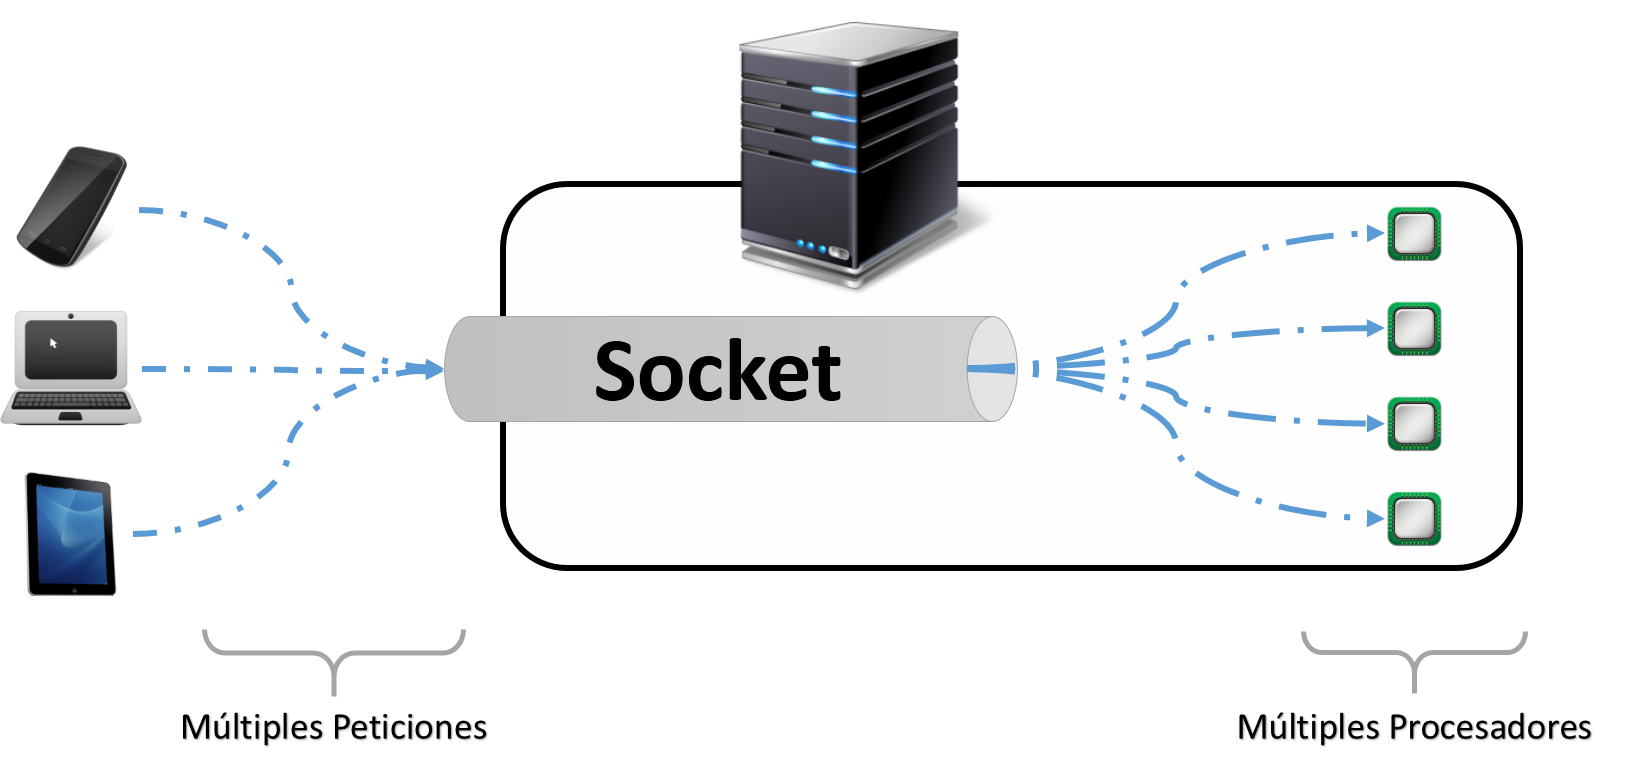
\includegraphics[scale=0.45]{imagenes/conf_multi_thread}
	\caption{Esquema de procesamiento multi-thread en un servidor con 4 procesadores reales, empleando un thread por procesador. Escenario que en teoría, supone un mejor desempeño general, más no lo consigue en la práctica.}
	\label{fig:multi_thread}
\end{figure}

Inspirados en la consistencia del argumento teórico detrás de la propuesta anterior, varias instituciones han evaluado este enfoque de procesamiento \cite{url:facebook, paper:toshiba}, pero con resultados poco alentadores. La experiencia de NIC Chile es un buen ejemplo del problema detectado. Aprovechando su infraestructura en pos de mejorar sus propios servicios, NIC Chile (Administrador del Top Level Domain \emph{.CL}) evaluó un diseño multi-hilos en el procesamiento de consultas DNS a sus servidores, a fin de lograr una mejora de performance en su procesamiento DNS tal y como el diseño teórico anterior plantea sin sospechar el resultado real. Al incorporar paralelismo, el rendimiento final en la práctica no estuvo ni cerca de las proyecciones esperadas, y lejos de reducirse, los tiempos de procesamiento aumentaron con respecto al esquema sin multi-hilos, ello aun cuando no existían indicios de sobrecarga en las máquinas.

\subsection{Validación del Problema}

Para ilustrar el interés del problema antes descrito es necesario validar la persistencia del mismo en escenarios actuales, que corroboren la persistencia del problema en escenarios de interés, como viene siendo el caso de servidores DNS. Para ello, se realizará un estudio de la situación actual del escenario multithreading separando los dos contextos antes mendionados: \textbf{Hardware}, probando el rendimiento en sistemas de arquitecturas de hardware diferente, y \textbf{Software}, probando el rendimiento en escenarios de ejecución basados en distitnas versiones del kernel de Linux.

\subsubsection{Validación en Distintas Arquitecturas}

\subsubsection{Validación en Distintas Versiones de Kernel de Linux}

AKA una linea del tiempo de los releases del kernel


\subsection{Hipótesis del Problema}
Las sospechas iniciales acerca de éste problema apuntan a que probablemente el defecto se esconda en el núcleo del sistema operativo. Desde su versión 2.6, el kernel de Linux incorporó capacidad de procesamiento simétrico multiprocesador (\emph{Symmetric Multi-Processing - SMP}), con esto el scheduler de tareas transfirió los hilos de ejecución paralelos al mismo núcleo del sistema, con el costo de tener que implementar protección para áreas completas de código y estructuras a fin de evitar modificaciones concurrentes. Para ello, Linux provee diversas primitivas de sincronización mencionadas en secciones anteriores a disposición de los programadores. Sin embargo, el módulo de redes del kernel de Linux data de versiones previas a la 2.6 que suponían entre sus recursos a monoprocesadores y que, por lo tanto, no consideraban operaciones simultáneas con múltiples procesadores como se consiguió con \emph{SMP}.

La sospecha inicial apunta a que probablemente, el efecto encontrado al evaluar diseños como el de la ilustración \ref{fig:multi_thread} es precisamente reflejo de un problema a nivel del kernel, donde alguna estructura de sincronización de bajo nivel está presentando un problema de contención, que se traduce en una serialziación de acceso, o similar, y que repercute en tiempos muertos en casos de concurrencia.

Hablar de las sospechas dadas por google en sus enfoques de contencion y que justifican reuseport.